\subsection{Performance Analysis}
After hyperparameter selection, with 3 different loss functions, the final configuration is trained for 50 epochs with early stopping of patience 10.Training statistics are recorded including loss history and validation accuracy.
\subsubsection{Performance And Accuracy}
\begin{table}[H]
\centering
\caption{Accuracy and mIoU performance}
\label{tab:loss_ablation}
\begin{tabular}{l c c} % 修改 1：原本有两列数据（Accuracy 和 mIoU），加上表头共 3 列，需要改为 l c c
\toprule
Loss Function & Validation Accuracy & Validation mIoU \\
\midrule
CrossEntropy Loss & 0.8139 & 0.5733 \\ % 修改 2：修正拼写 CrossEntropy -> CrossEntropy
Dice Loss & 0.8173 & 0.5862 \\
Combined Loss & 0.8166 & 0.5919 \\ % 修改 3：修正拼写 Conbined -> Combined
\bottomrule
\end{tabular}
\end{table}

\subsection{Analysis of Table~\ref{tab:loss_ablation}}
\subsubsection{Superiority of Dice Loss and Combined Loss}
As demonstrated in Table~\ref{tab:loss_ablation} and the training curves, both \textit{Dice Loss} and \textit{Combined Loss} outperform the standard \textit{Cross-Entropy Loss} by a significant margin, particularly in terms of mIoU. Specifically, Compared to the CE baseline (0.5733), Dice Loss and Combined Loss improve the mIoU by 1.29\% and 1.86\% respectively. 

The underlying reasons for this superiority are analyzed as follows:
\begin{itemize}
    \item \textbf{Class Imbalance} The Oxford-IIIT Pet dataset exhibits a severe pixel-level class imbalance, where the background pixels dominate the majority of the image, while the pet boundary pixels occupy only a tiny fraction. Standard Cross-Entropy loss treats each pixel equally, leading the gradients to be heavily dominated by the background class. Consequently, the model biases towards majority classes to achieve a high pixel accuracy while sacrificing smaller, critical structures.
    \item \textbf{Optimization of Regional Overlap} In contrast, Dice Loss is formulated based on the Dice coefficient, which directly measures the regional overlap between the prediction $P$ and ground truth $G$:
    \begin{equation}
        \mathcal{L}_{\text{Dice}} = 1 - \frac{2 |P \cap G|}{|P| + |G|}
    \end{equation}
    Because the denominator normalizes the overlap by the total area of both regions, Dice Loss is immune to class scale imbalances. Focusing on the global structure of foreground objects.
\end{itemize}


\subsubsection{Trade-off Between Accuracy and mIoU: Dice Loss vs. Combined Loss}
Another worth mentioning phenomenon observed in Table~\ref{tab:loss_ablation} is that while \textit{Dice Loss} achieves a slightly higher Validation Accuracy (0.8173) than \textit{Combined Loss} (0.8166), its Validation mIoU (0.5862) is notably lower than that of the Combined Loss (0.5919). 

This instance stems from how Accuracy and mIoU weigh segmentation errors:
\begin{itemize}
    \item \textbf{The Limitation of Pure Dice Loss at Boundaries:} Dice Loss focuses entirely on maximizing the regional intersection. However, during the late stages of training from scratch, the gradient of Dice Loss can become unstable or vanish when the predicted mask highly overlaps with the target. This prevents the model from fine-tuning ambiguous boundaries or pixels with low confidence, leading to suboptimal segmentation on fine details like pet outlines, which drags down the mIoU score.
    \item \textbf{The Synergistic Effect of Combined Loss:} \textit{Combined Loss} solves this bottleneck by integrating Cross-Entropy and Dice Loss. In this formulation, Dice Loss quickly captures the global shape during the early training phase, while Cross-Entropy penalizes pixel-level misclassifications at the boundaries in the later phase. Although this strict pixel-level penalty slightly compromises the overall global Accuracy (by a negligible 0.07\%), it heavily refines boundary precision, thereby yielding the highest mIoU across all configurations.
\end{itemize}

\subsubsection{Further Insights: Training Dynamics and Optimization Stability}
Beyond the final numerical results, the training dynamics provide deeper insights into the loss engineering process, the dice loss and combined loss offer a more smooth optimization path, which will be illustrated later.


\subsubsection{Training Dynamics and Optimization Stability}
\begin{figure}[H]
    \centering
    % 第一张子图 (a)
    \begin{subfigure}[b]{0.45\textwidth}
        \centering
        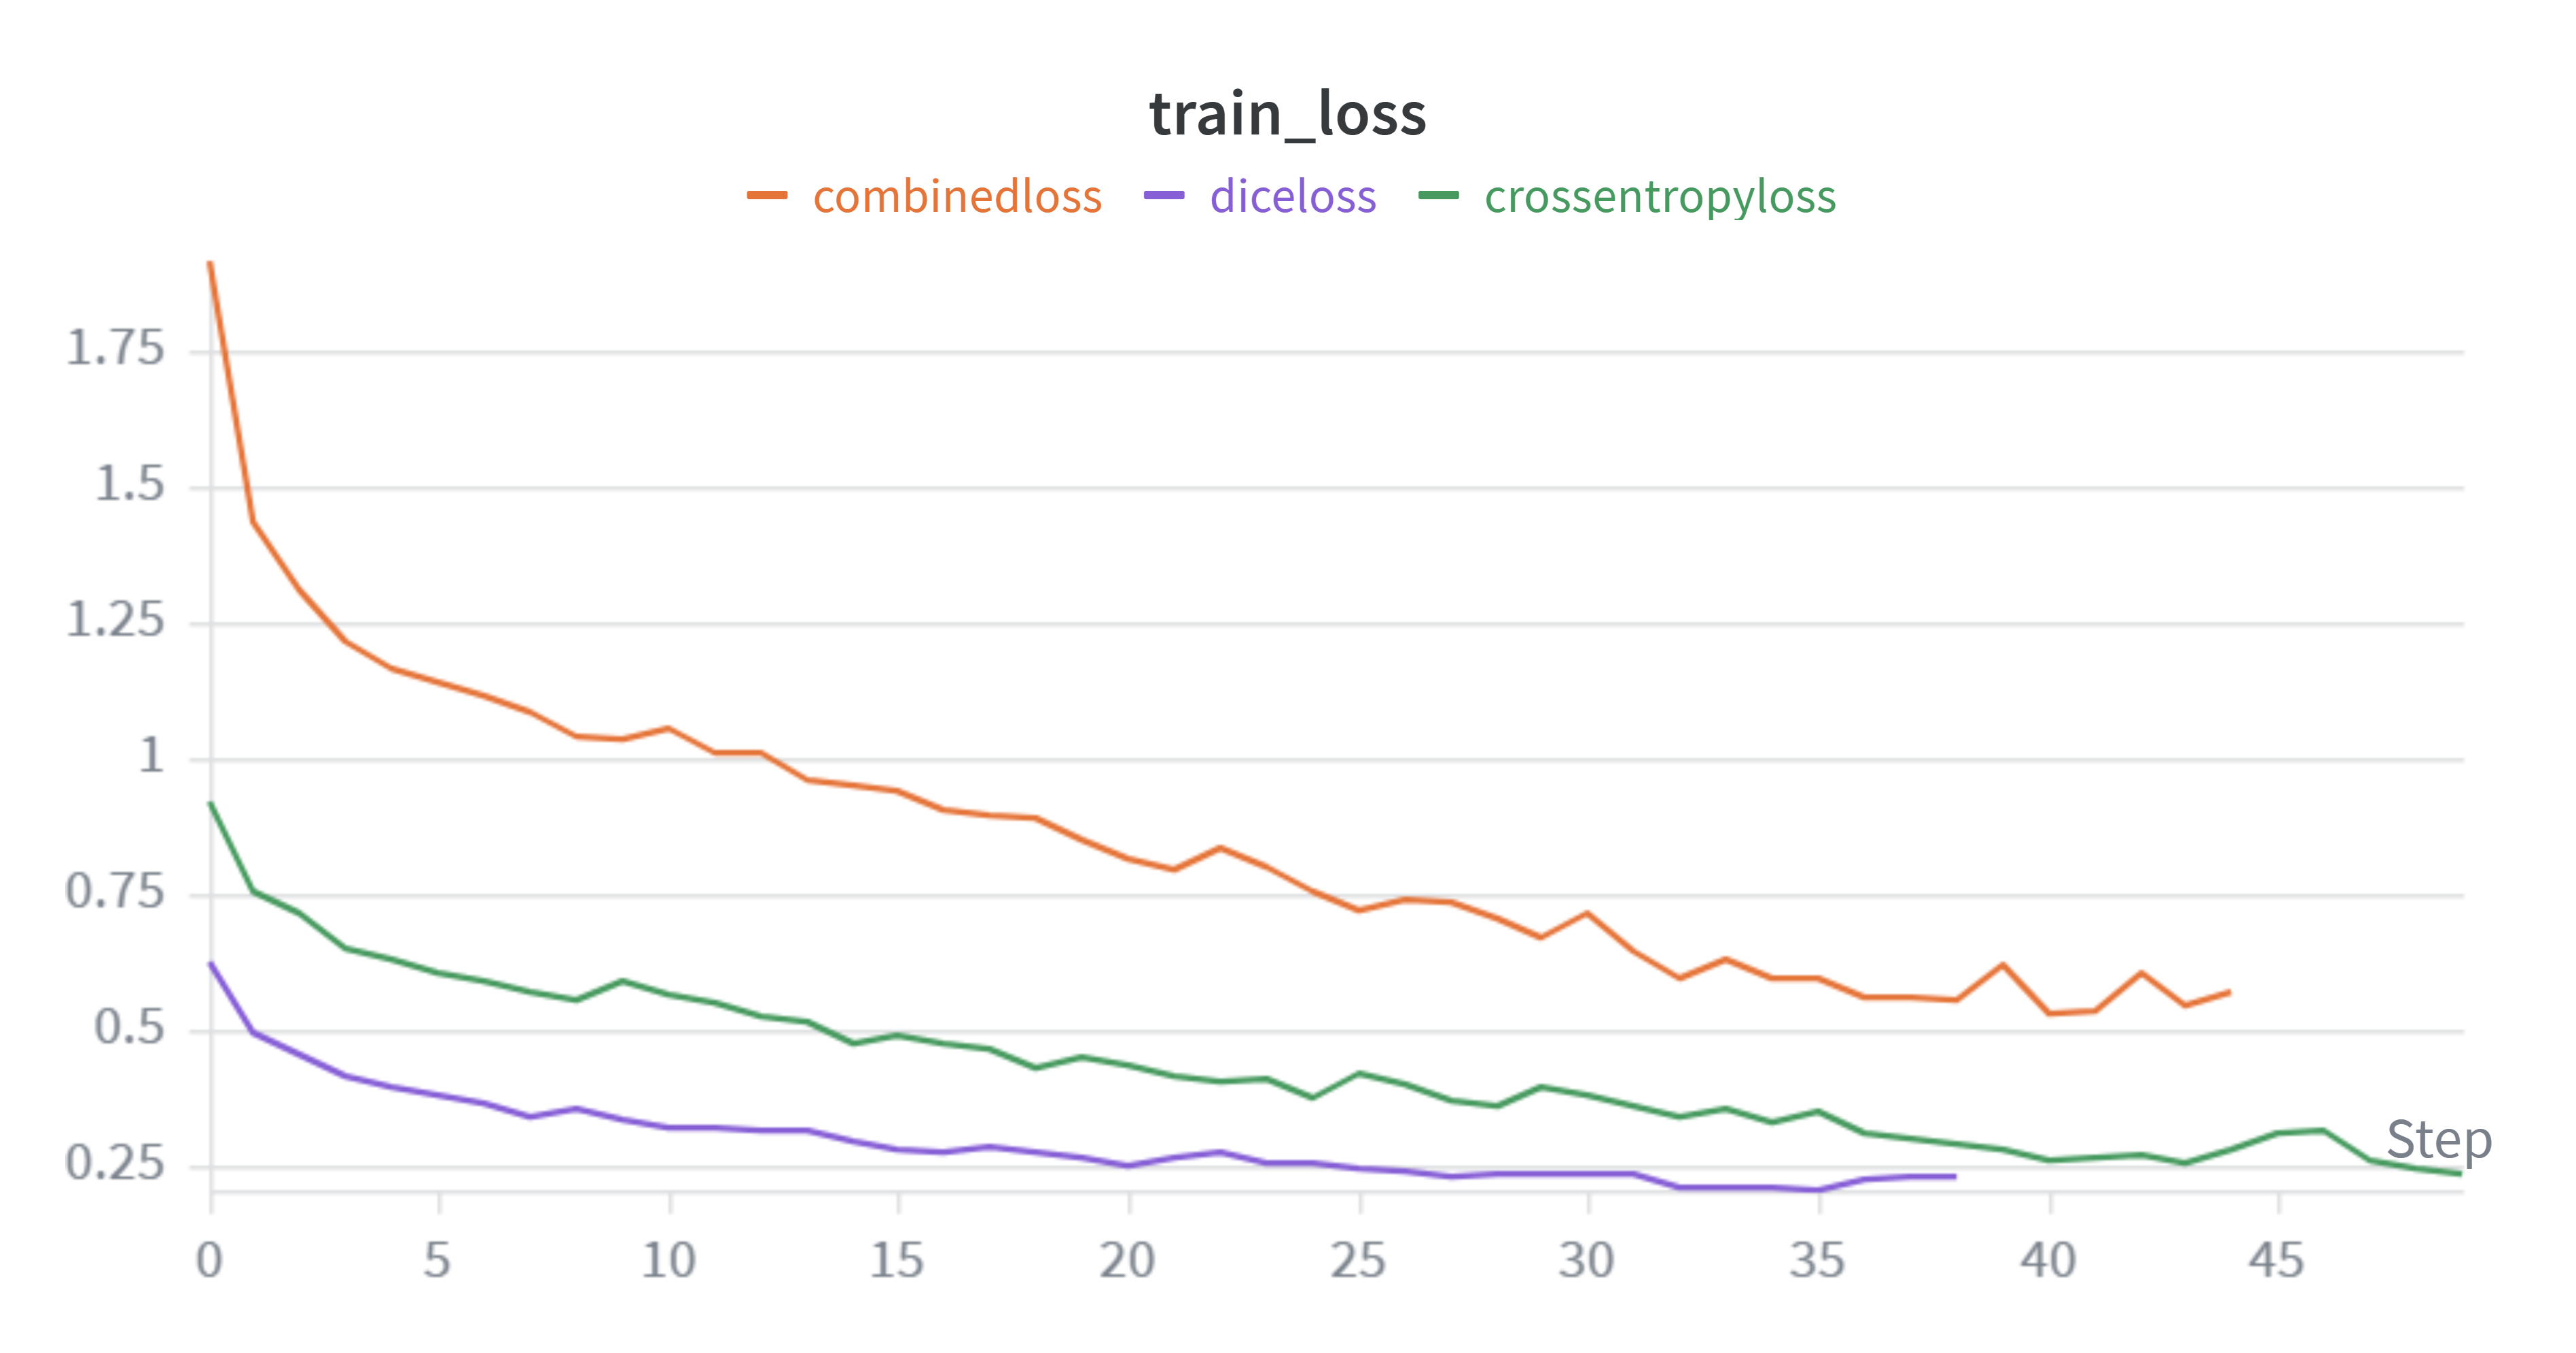
\includegraphics[width=\textwidth]{figures/task3/trainloss.png}
        \caption{Train Loss}
        \label{fig:train_loss}
    \end{subfigure}
    \hfil % 两张图之间的横向间距
    % 第二张子图 (b)
    \begin{subfigure}[b]{0.45\textwidth}
        \centering
        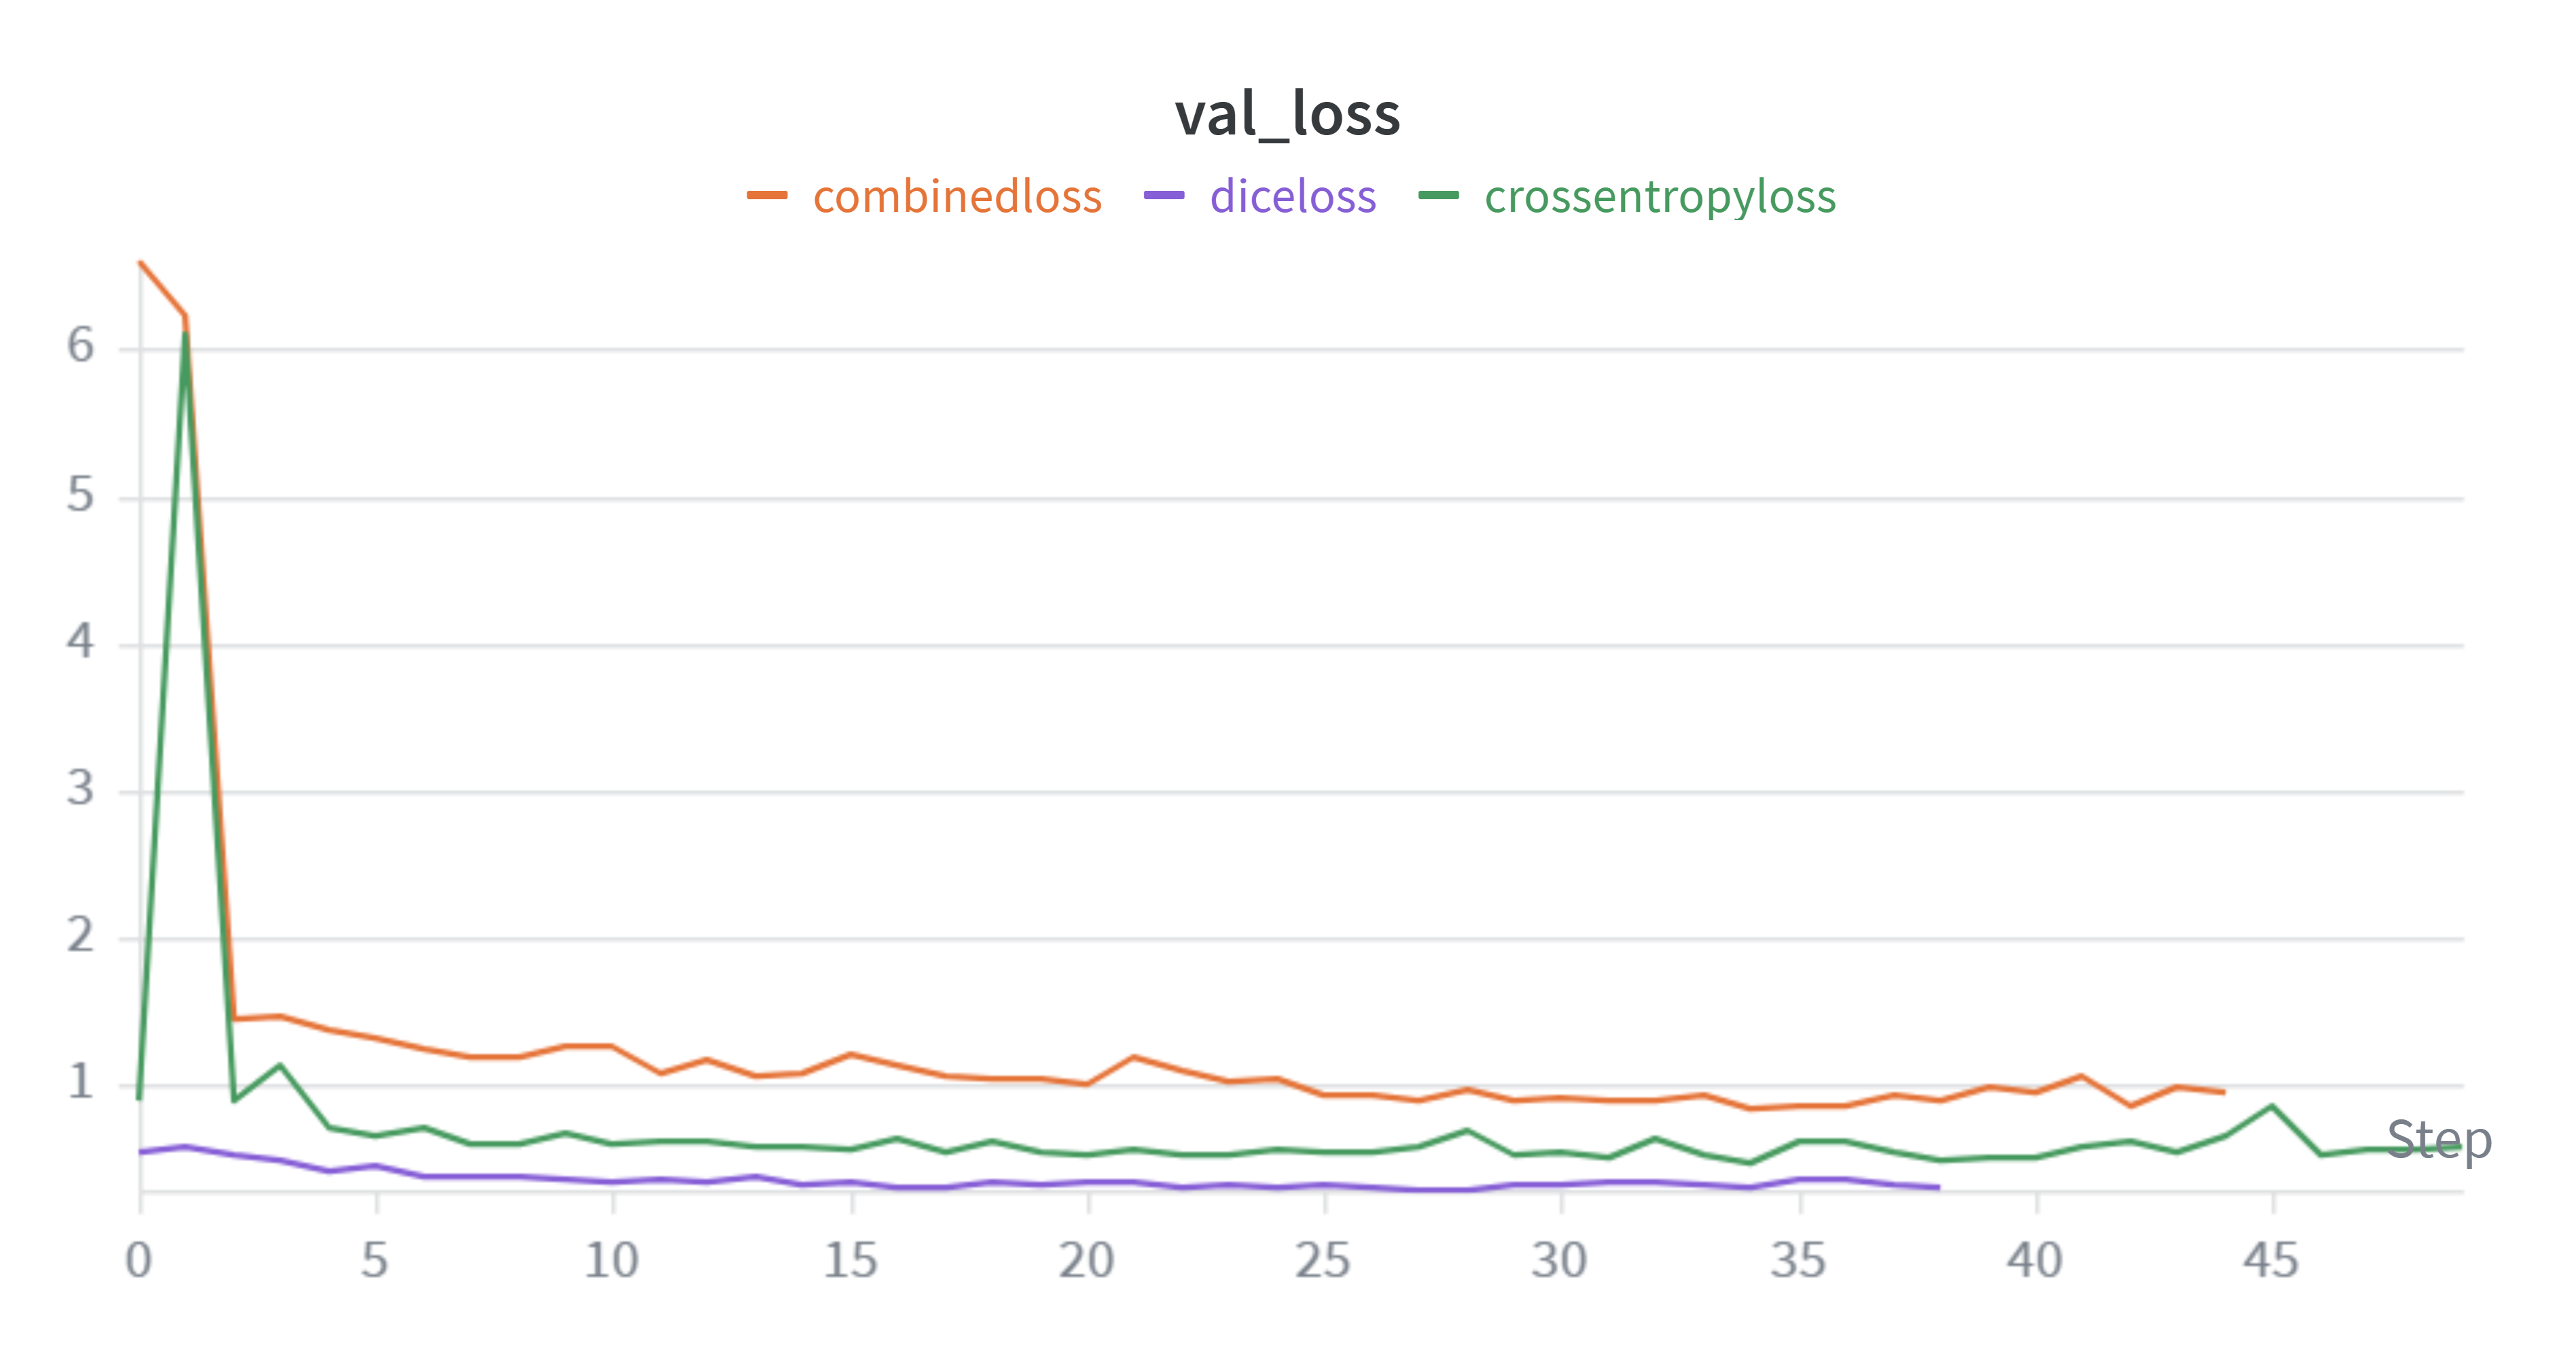
\includegraphics[width=\textwidth]{figures/task3/valloss.png}
        \caption{Val Loss}
        \label{fig:val_loss}
    \end{subfigure}
    
    \vspace{0.3cm} % 上下两行之间的纵向间距，防止挤在一起
    
    % 第三张子图 (c)
    \begin{subfigure}[b]{0.45\textwidth}
        \centering
        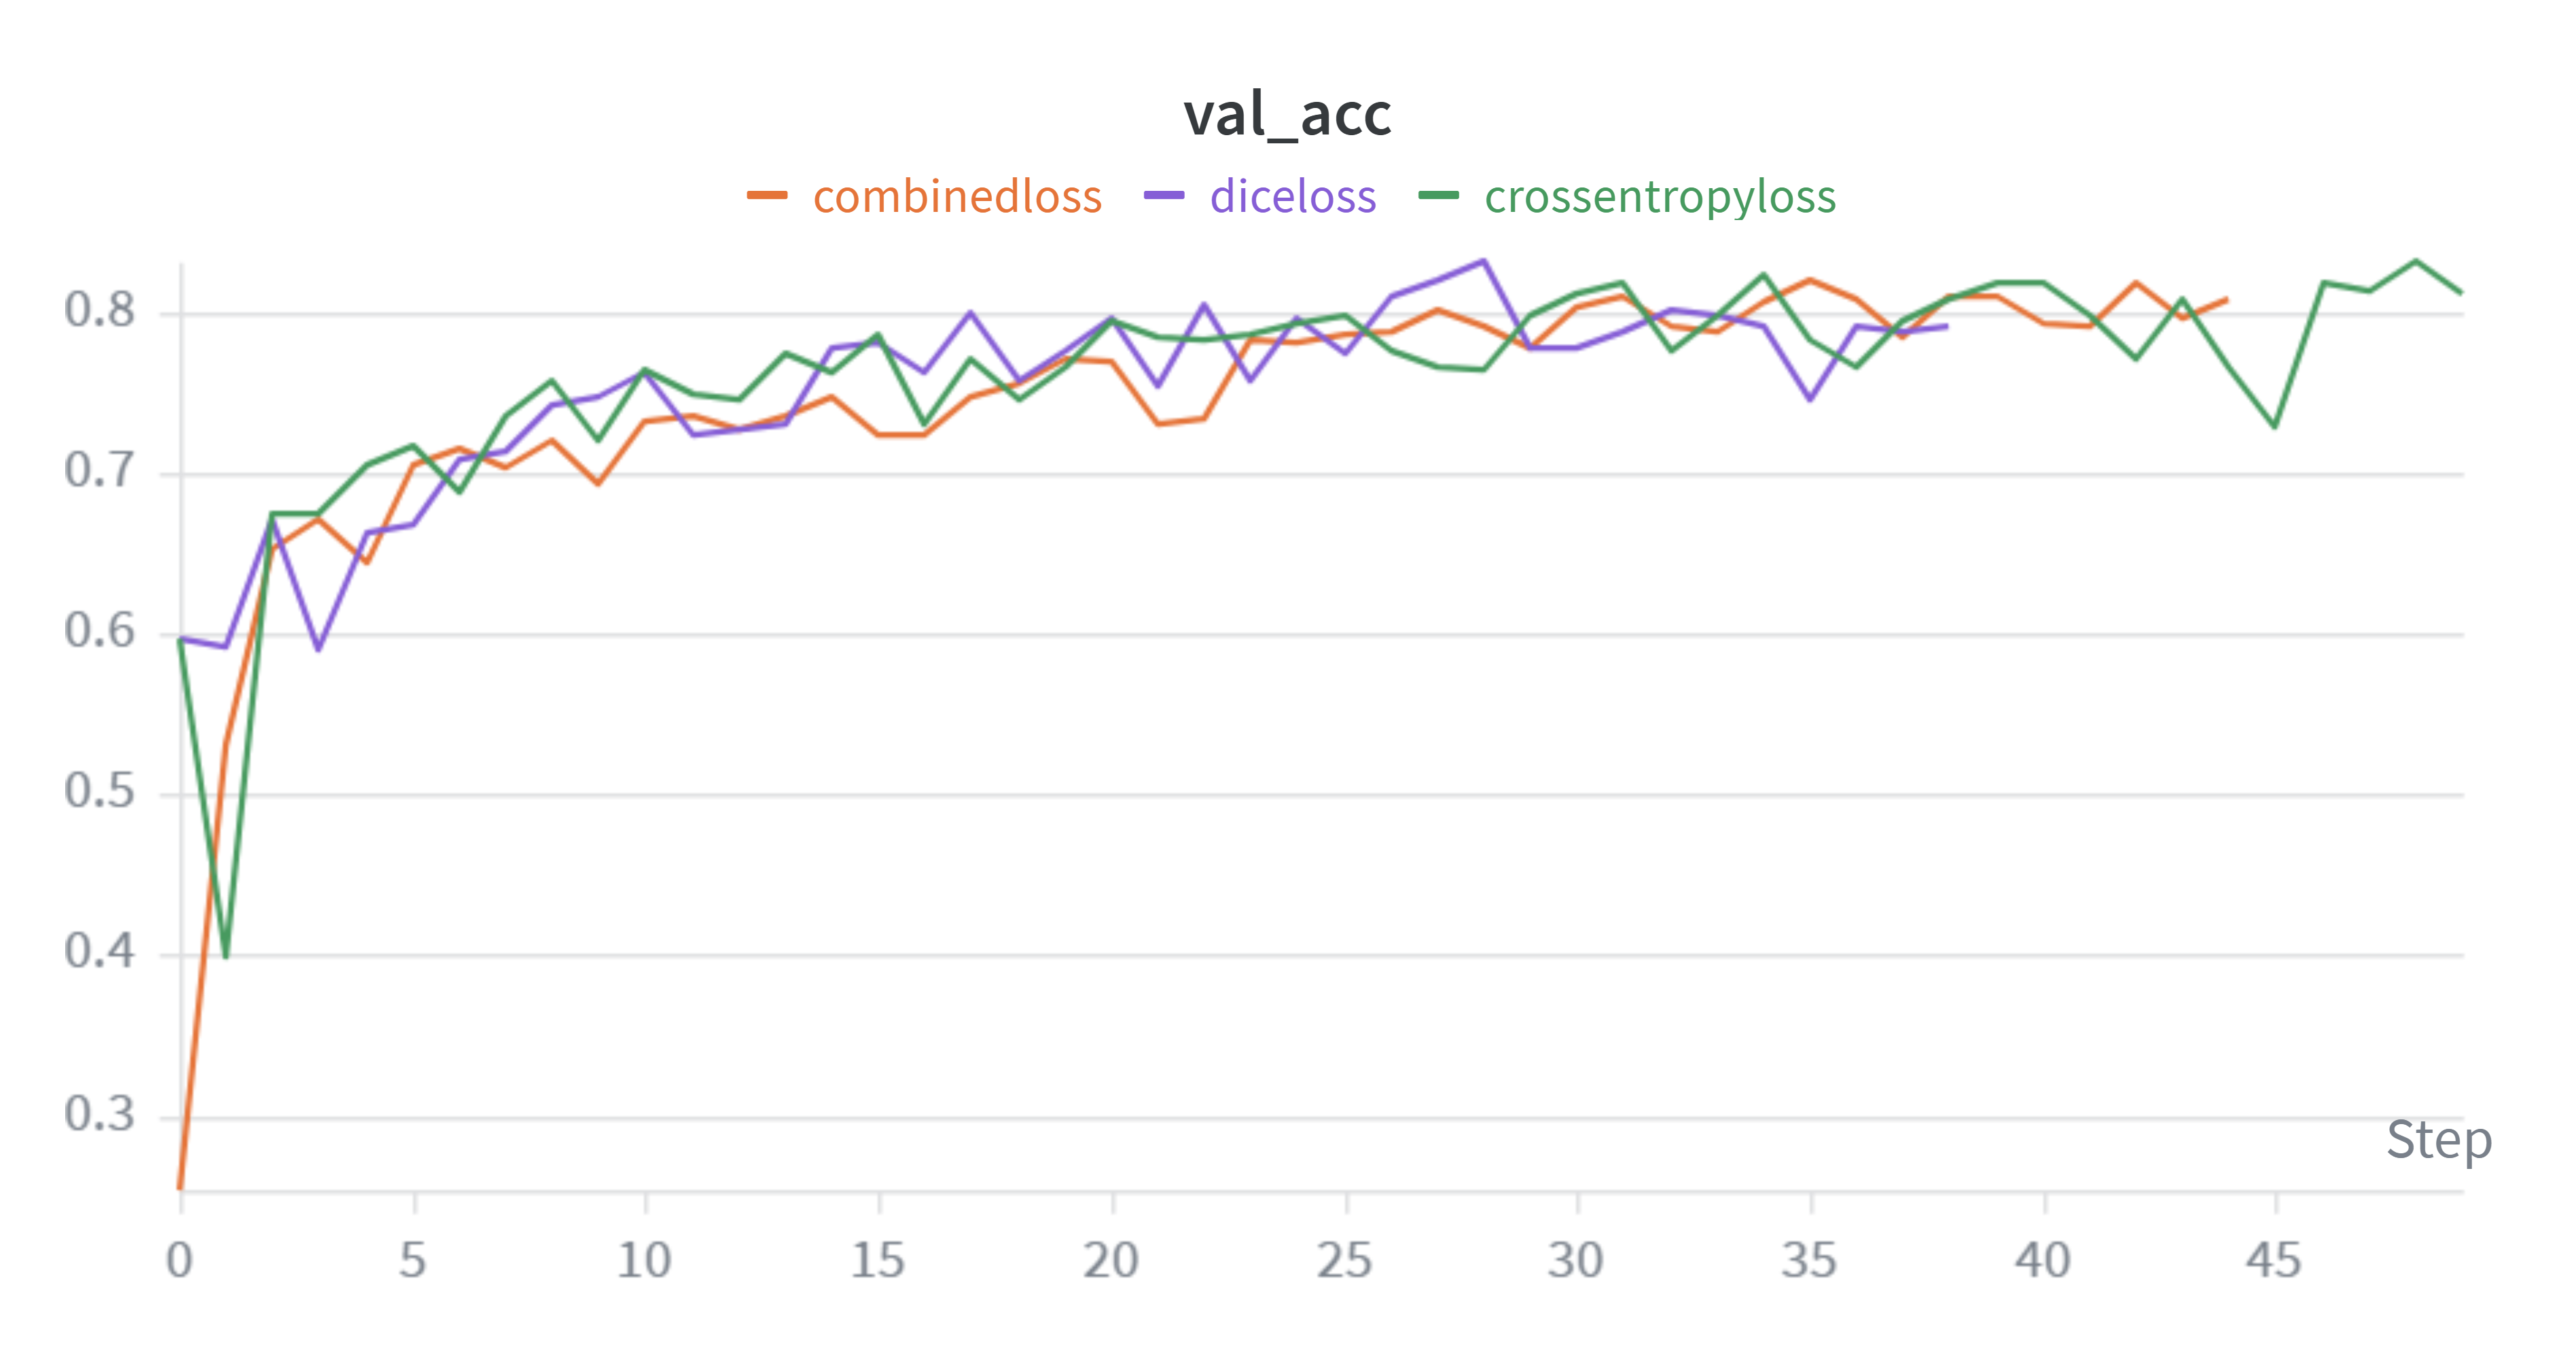
\includegraphics[width=\textwidth]{figures/task3/valaccu.png}
        \caption{Val Accuracy}
        \label{fig:val_acc}
    \end{subfigure}
    

\end{figure}
As is shown in the above figures, the models with different loss functions show similar optimization behavior on the training set. Their training losses decrease at comparable rates, and their training accuracies converge to nearly the same level.

Also, it's easy to see in Figure(a) that the orange curve is close to the sum of the remaining two curves, which is consistent with our definition.

It's worth mentioning that in Figure(b), the green curve(CrossEntropy Loss) has a very sharp spike at the very beginning of training (the first two steps), surging to around 6.0, before quickly dropping back and remaining stable in subsequent training sessions. While the other 2 curves have smooth overall performance with no violent fluctuations. This is because: Cross-entropy focuses on the "accuracy of pixel classification." If the model mispredicts a rare category in a large area, it will trigger a severe penalty.Dice Loss focuses on region overlap. Because it considers the sum of the predicted and ground truth regions in its denominator, it is naturally immune to pixel imbalance. Therefore, its training and validation processes are more robust and smooth.

\subsubsection{Confution Matrix Analysis}
\begin{figure}[H]
    \centering
    
\includegraphics[width=0.7\textwidth]{figures/task3/confusion_matrix.png} 
    \caption{confusion matrix trained with Combined Loss} 
    \label{fig:confusion_matrix}
\end{figure}

To further investigate the performance of model, the confusion matrix on the validation set is illustrated in Figure~\ref{fig:confusion_matrix}. 

The most frequent confusion pairs include:
\begin{itemize}
    \item \textbf{Contour $\rightarrow$ Background (0.2999):} Approximately 30.0\% of the actual pet boundary pixels are erroneously predicted as background.
    \item \textbf{Contour $\rightarrow$ Pet Body (0.2128):} Around 21.3\% of the actual contour pixels are misclassified as part of the pet's core region.
    \item \textbf{Pet Body $\rightarrow$ Background (0.1718):} About 17.2\% of the foreground pet pixels are missed and assigned to the background environment.
\end{itemize}

These errors are mainly caused by the spatial ambiguity of the transition region. Specifically, the \textit{Contour} class represents an extremely thin, line-like structure enclosing the pet. Since boundaries are only a few pixels wide, even a minor spatial shifting or thickness mismatch during U-Net's upsampling phase will drift the predictions into either the \textit{Background} or the \textit{Pet Body} domain, resulting in a low diagonal accuracy of 0.4873 for the boundary class. 

Furthermore, the confusion between \textit{Pet Body} and \textit{Background} (0.1718) is primarily driven by local visual similarities, such as pets with fur colors resembling background like rugs or grass. The confusion matrix therefore suggests that the remaining segmentation difficulty is largely caused by the fine-grained edge uncertainty and severe pixel-level class scale variations, rather than a failure in the model's structural optimization or gradient convergence.
\subsubsection{Error Case Analysis}
Representative failure cases are shown as follow:

\begin{figure}[H] % [p] 表示将这些大图集中放在独立的一页，避免打乱正文排版
    \centering
    
    % 第一张大图
    
\includegraphics[width=\textwidth]{figures//task3/example1.png} % 替换为你的第一张图片文件名
    \caption{a}  
    \label{fig:case1}
    \vspace{0.25cm} % 在图片之间留出一点垂直间距

    % 第二张大图
    
\includegraphics[width=\textwidth]{figures//task3/example3.png} % 替换为你的第二张图片文件名
    \caption{b}  
    \label{fig:case2}
    \vspace{0.25cm}

    % 第三张大图
    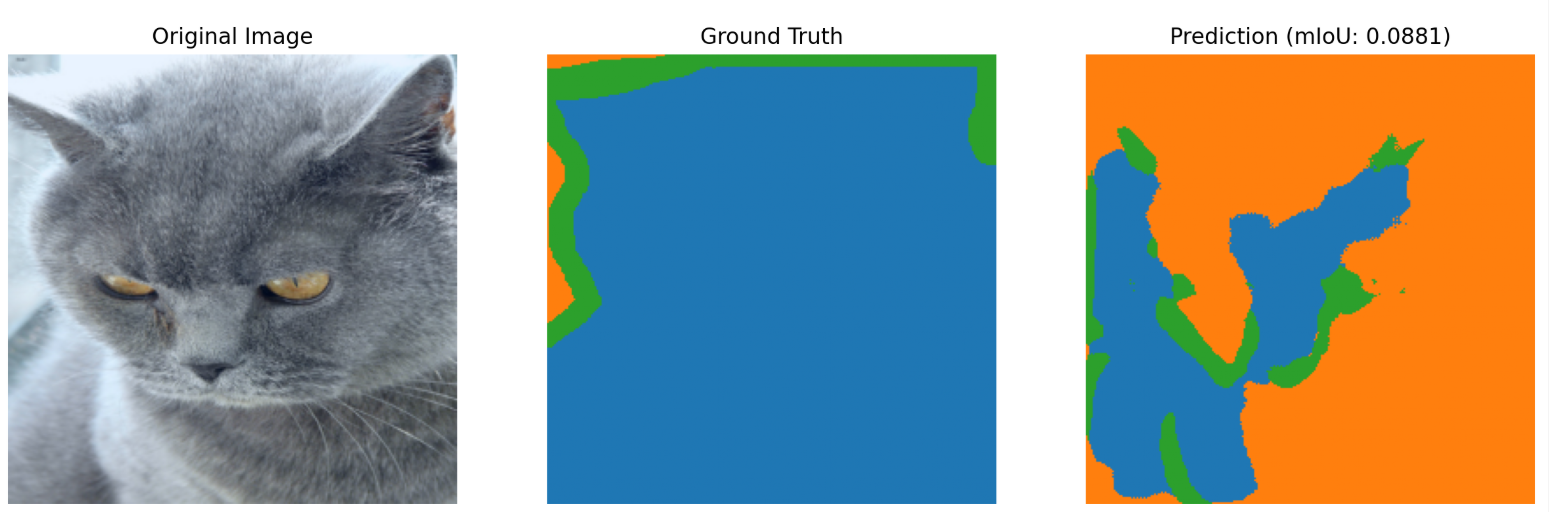
\includegraphics[width=\textwidth]{figures//task3/example2.png} % 替换为你的第三张图片文件名
    \caption{c}    
    \label{fig:case3}
    
\end{figure}
As observed in Figure~\ref{fig:case1}(a), the network struggles with complicated semantic transitions. The delicate contour around the animal's neck is completely mispredicted as the core \textit{Pet Body} due to the issue of light and shadow. Meanwhile, the lower legs are largely misclassified into either the \textit{Background} or a\textit{Contour} region. This directly corresponds to the outcome of the confusion matrix, where 21.28\% of true contour pixels drift into the body domain,17.17\% of true body pixels and 29.99\% of true contour pixels drift into the background domain, demonstrating that the model still experiences spatial uncertainty on slender structures.

In Figure~\ref{fig:case2}(b), a noticeable geometric deformation occurs along the overall outline of the cat. The root cause lies in the low visual contrast and texture similarity between the cat's orange fur and the background wooden floor. Due to the absence of pre-trained weights, the randomly initialized encoder lacks the high-level semantic prior needed to distinguish similar object boundaries, thus bringing bad performance.

Figure~\ref{fig:case3}(c)presents a catastrophic failure case with an exceptionally low mIoU of 0.0881. This specimen is highly unconventional as it features a close-up shot where the cat's head occupies nearly the entire field of view, leaving only a fractional background strip on the left edge. Because the model was trained from scratch, it heavily overfits to the global spatial prior that a pet must be surrounded by a dominant background. When confronted with this extreme target scale variation, the spatial context mechanism of U-Net collapses, mistakenly treating the homogeneous gray fur as background and fracturing the body into fragments.